\documentclass[]{article}

\usepackage{graphicx}
\usepackage{float}

%opening
\title{Visual Analytics \\ Practical 3}
\author{Michael Weisz}
\date{February 16 -- Hilary Term 2017 }
\begin{document}

\maketitle


\section*{Summary}
This report summarises my work on the third practical \emph{Parallel Coordinates Plots} as part of the \emph{Visual Analytics} course at Hilary Term 2017 at Oxford University.

I have attempted levels 1 - 3 with all the required functionality such as the reordering of axes, colour coding as a tool for grouping data, and brushing. The subtleties of each level including the relevant excerpts of the sourced code are described in more detail in the corresponding sections. 

For the visualisations I used the \emph{D3.js} 
% TODO add link to d3 as footnote
charting library. I addition, I made use of the following existing examples in the \emph{D3} repository.

% TOOD links and names to examples*
* 



\section*{Level 1}
This level asked for a adaptation of an existing parallel coordinate plot in order to visualise the the data provided in \emph{WorldExconomy2015.xlsx}.

The resulting plot contain seven axes for each of the 19 data points and is shown below. 


\begin{figure}[t]

	\centering
	\makebox[\textwidth][c]{
	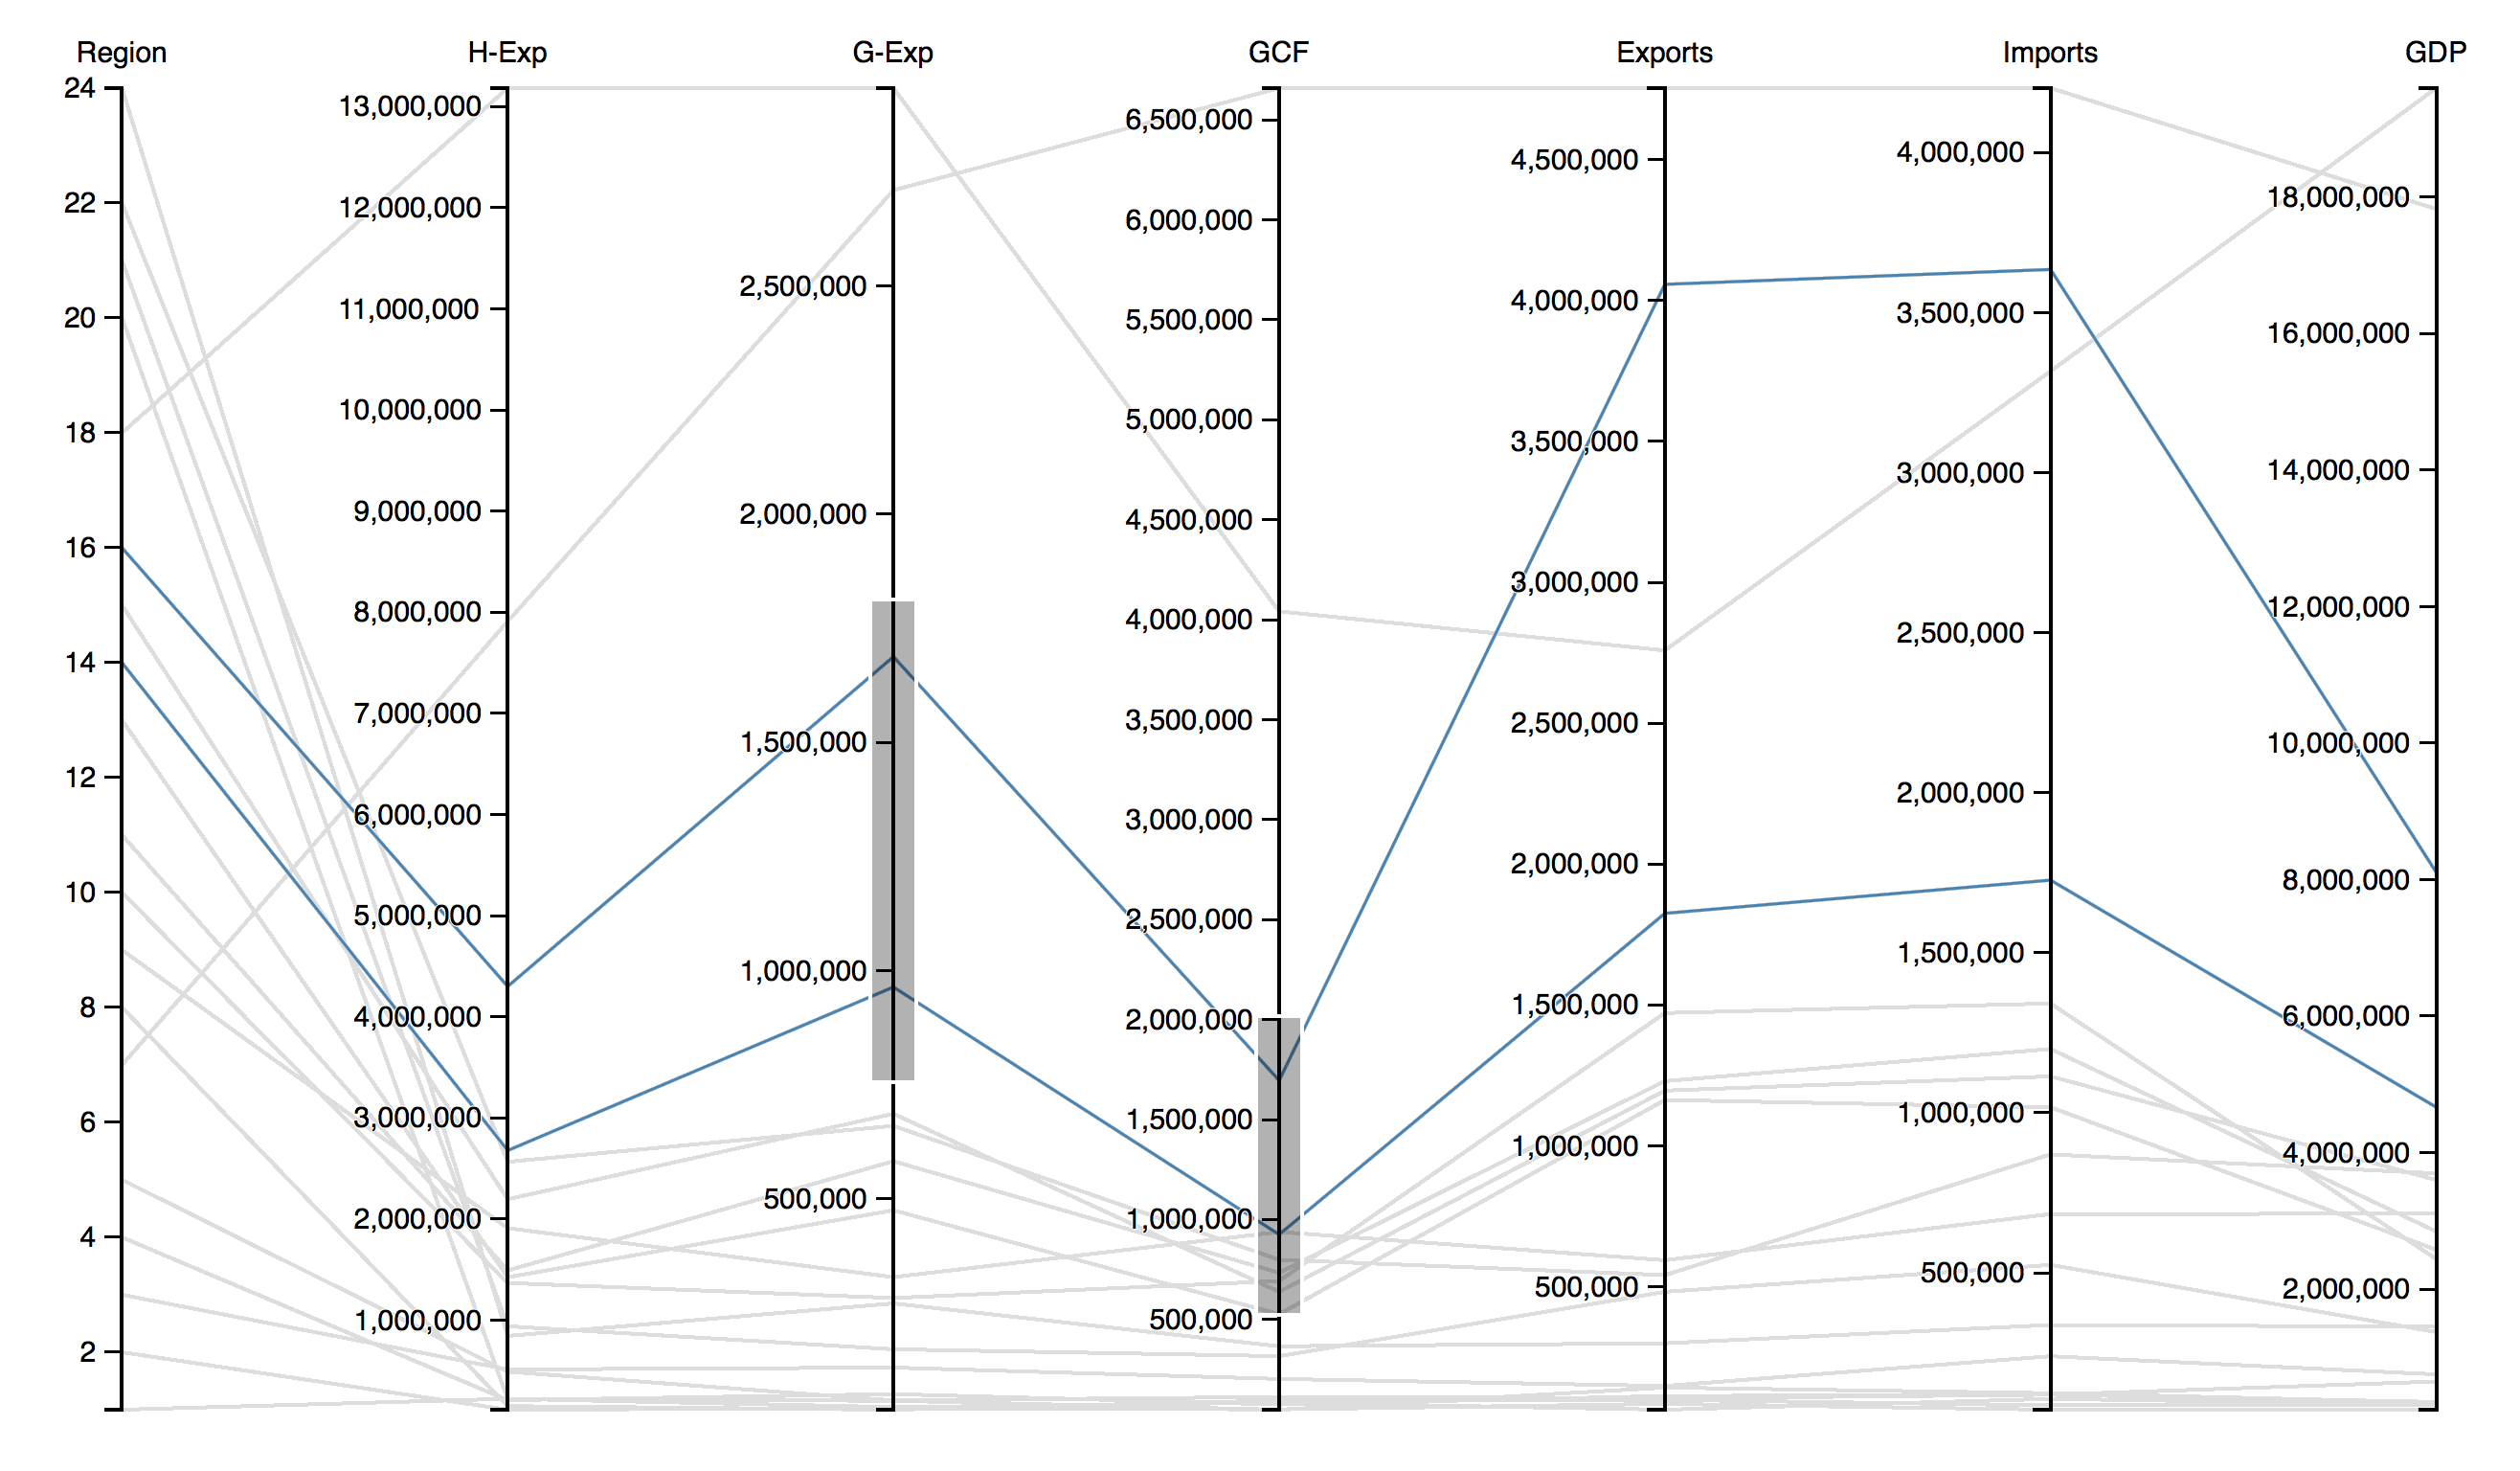
\includegraphics[width=1.3\textwidth]{img/level-1}
}
	\caption{Parallel coordinate plot for level 1 with brushing}
\end{figure}






\section*{Level 2}
This level asked to combine multiple datasets and colour code the lines in the graph depending on their \emph{region} dimension. 

In addition, the dataset contained categorical data for which the creation of the axes and the implementation of the brushing functionality had to be adapted.

\begin{figure}[t]
	
	\centering
	\makebox[\textwidth][c]{
		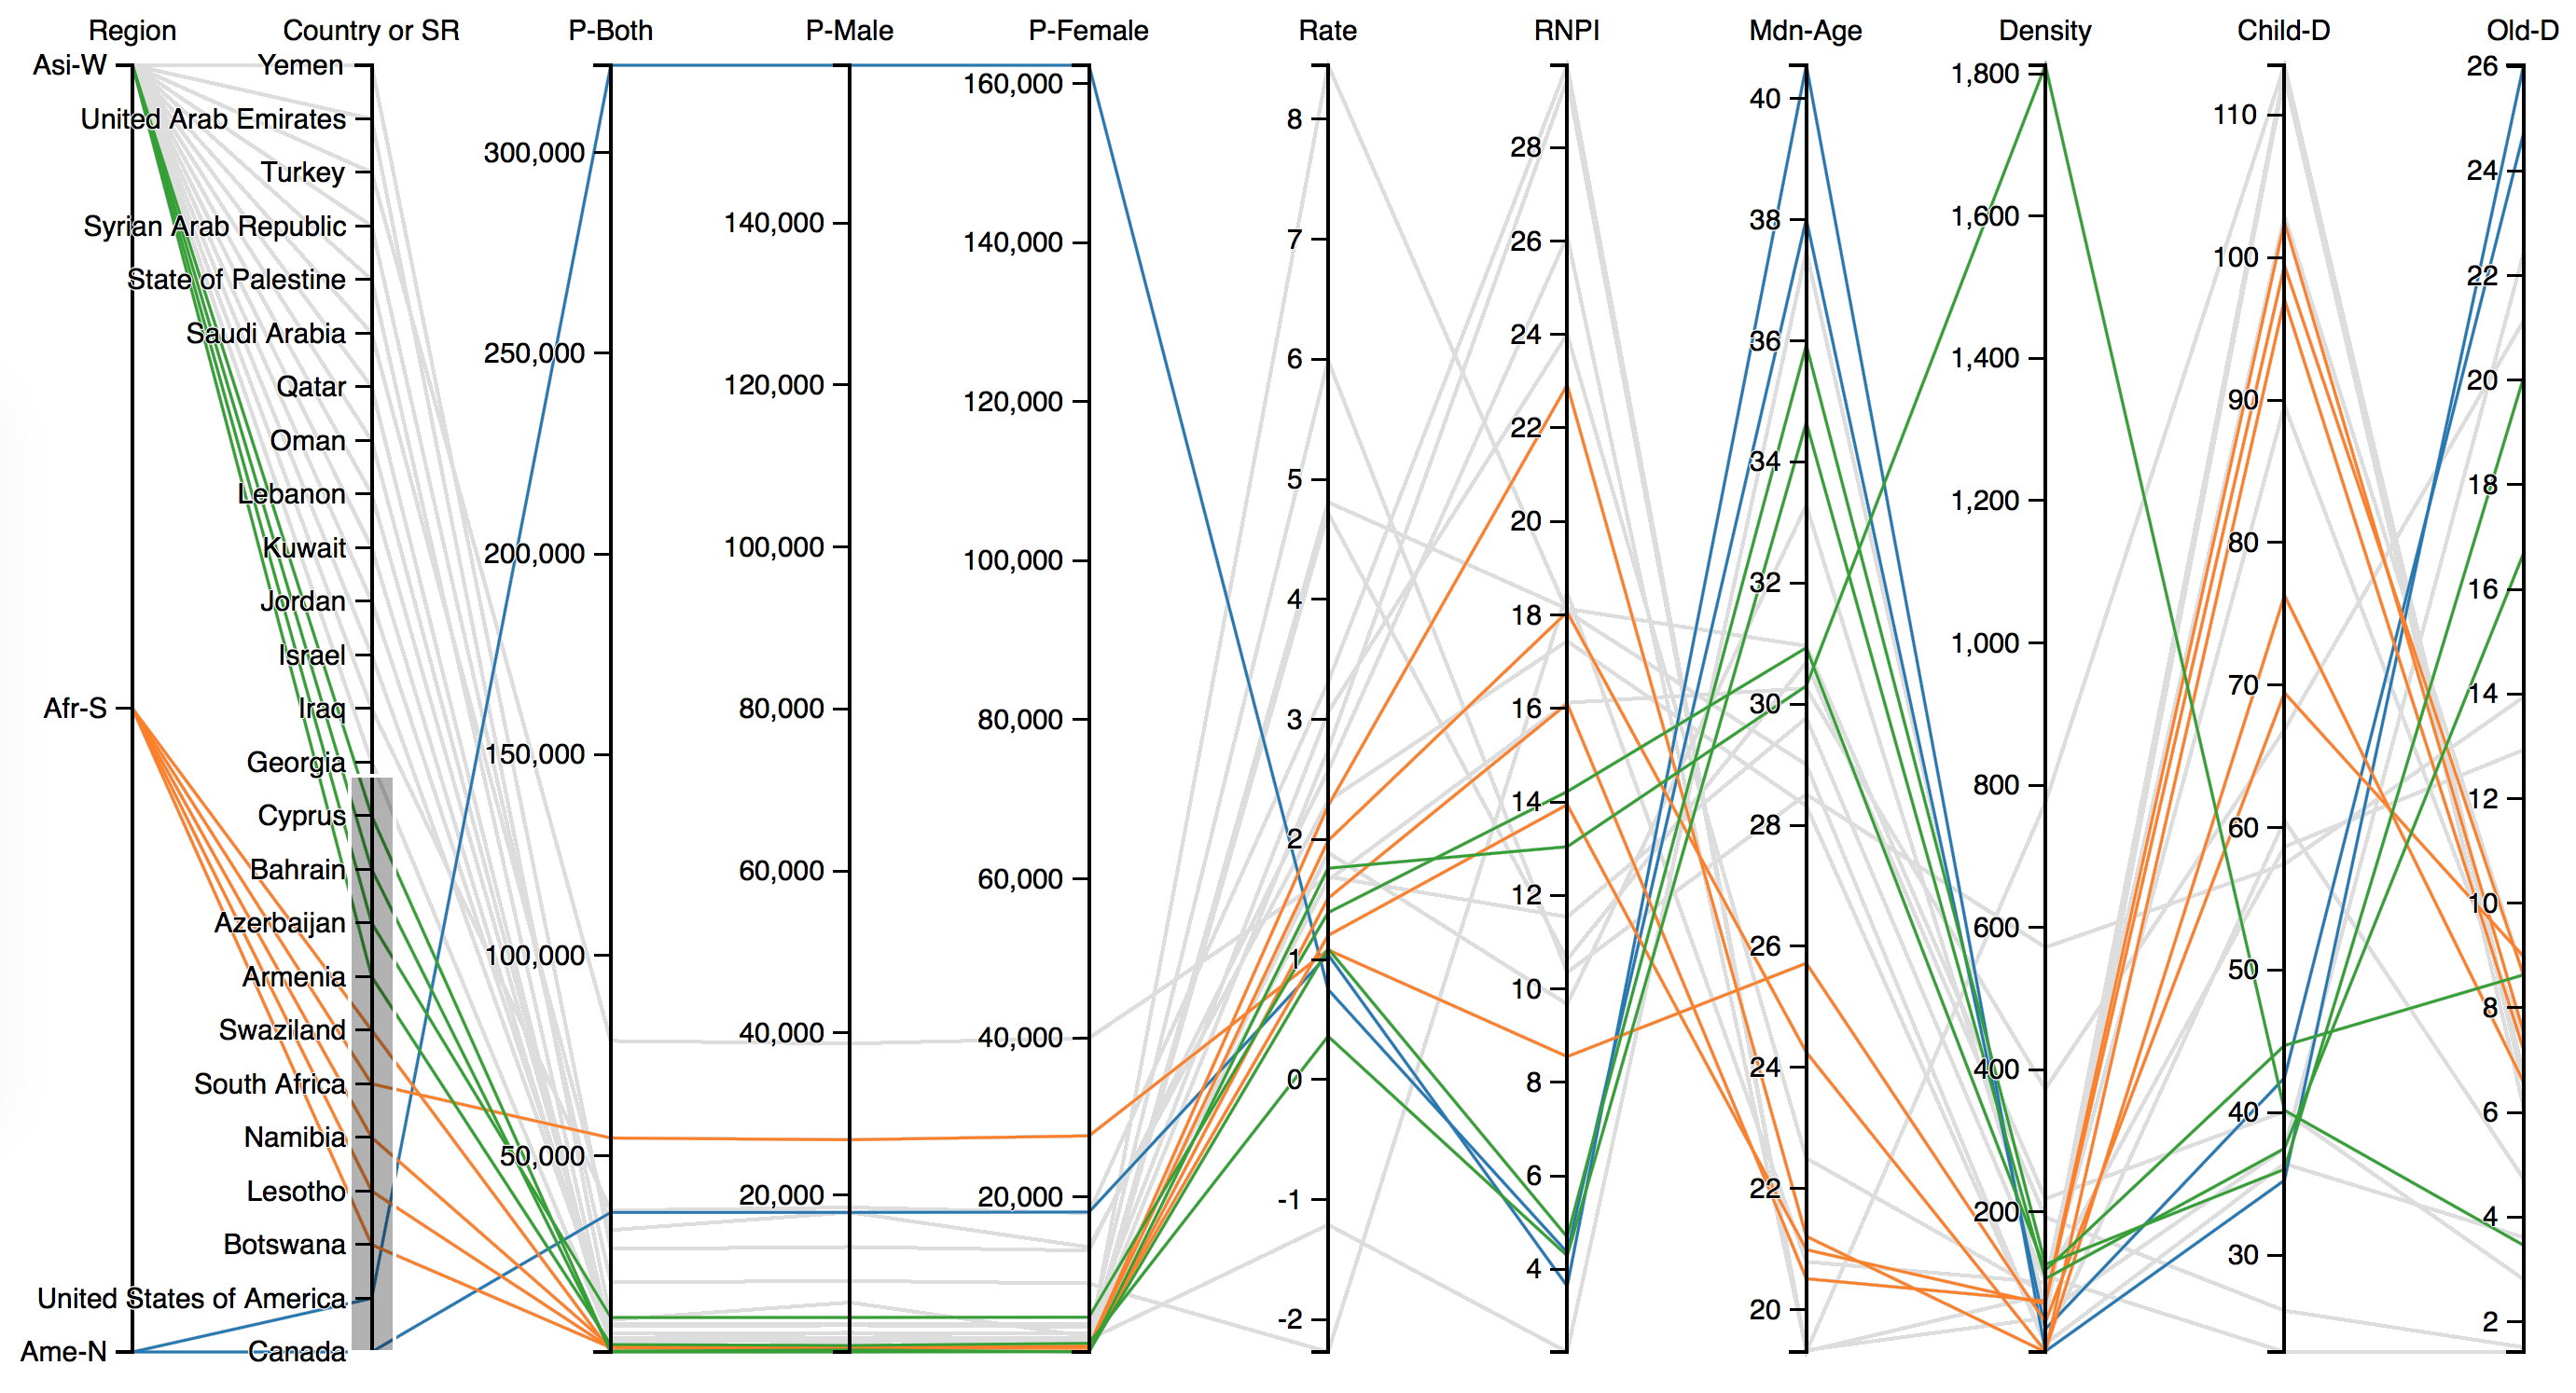
\includegraphics[width=1.3\textwidth]{img/level-2}
	}
	\caption{Parallel coordinate plot for level 2 with colour coding}
\end{figure}

\paragraph{Colour Coding} The following excerpt of the source code describes how the lines are drawn in different colours depending on their \emph{region} attribute. 
% TODO: Add source code for color coding

\paragraph{Ordinal Axes} The following excerpt of the source code shows how I implemented the creation of the different axis depending on their data type. 
% TODO: Add source code for Ordinal vs real-values axes


\paragraph{Brushing} The following excerpt of the source code shows how I implemented the brushing functionality which is handled differently depending on whether we have categorical or numerical data. 
% TODO: Check if 'numerical data' is the right term
% TODO: Add source code for brushing




\section*{Level 3}
The third and optional level asked for a way to show the temporal relationship of the \emph{world economy} dataset. One way to achieve this, is by offering a separate line chart which displays an aggregation (in this case, the average) when clicking on a certain axis in the parallel coordinate plot. 

\begin{figure}[t]
	
	\centering
	\makebox[\textwidth][c]{
		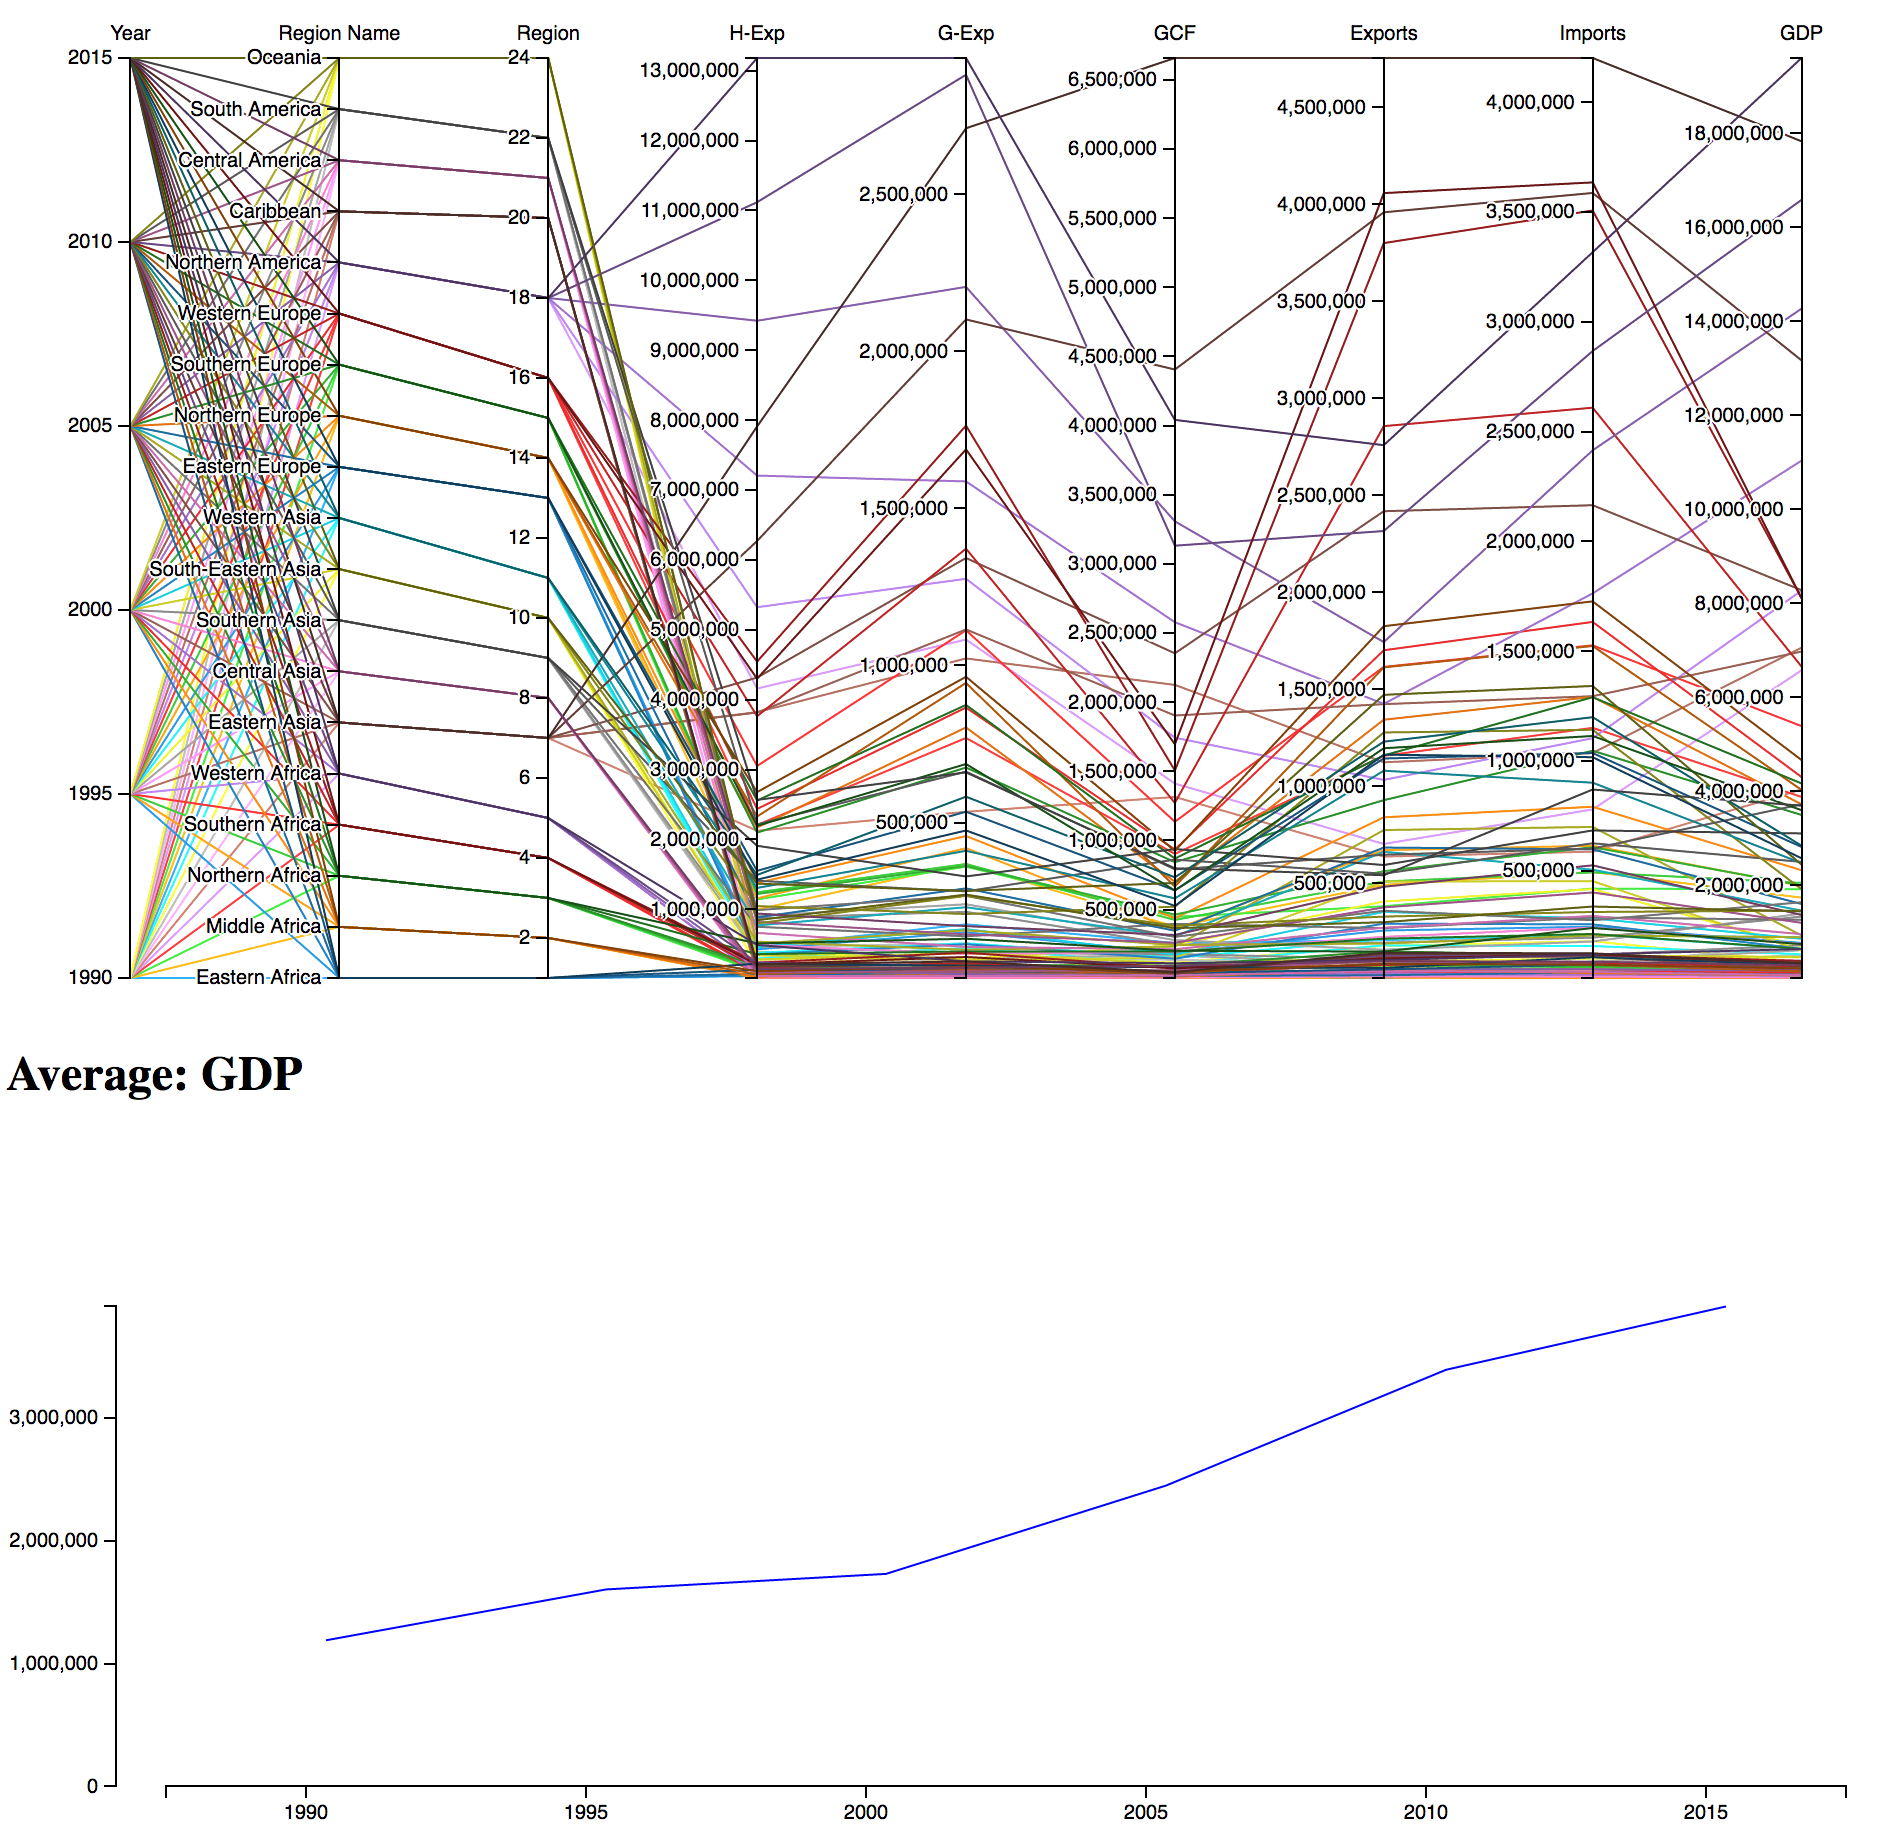
\includegraphics[width=1.3\textwidth]{img/level-3}
	}
	\caption{Parallel coordinate plot for level 3 with additional time series plot after clicking on axis}
\end{figure}

In addition, data points which have a common \emph{country} attribute are drawn in the same colour but with different saturations depending on their \emph{year} attribute (more recent is darker). 

The  


\end{document}
